\section{Supplementary results} \label{sec:annex_results}

%\subsection{Further results about trends in the level and distribution of household resources}\label{subsec:gics_by_period}

\subsection{Trends in the level and distribution of household resources}\label{subsec:aggregate_trends}

Table \ref{table:prctile} presents summary statistics on the distribution of household resources in the UK for a selection of years assessed using our four main measures: income with and without an imputed income from housing, and consumption with and without imputed consumption from housing. As discussed in Section \ref{section:measure}, all measures are given at the weekly level, equivalised for household structure using the OECD equivalence scale, and expressed in December 2009 prices using an appropriate variant of the RPI, and tables and figures refer to measures including the imputed consumption flow or implicit income from housing as IHC measures, and those excluding the same as XHC measures.  

There are some qualitative similarities between the distributions: each resource distribution, in each year, is positively skewed with the mean exceeding the median. But there are significant differences between the distributions, with Kolmogorov-Smirnoff tests rejecting equality of distributions at any plausible level in all years, for all pairwise comparisons of resource measures.\footnote{For all tests, p-values $\approx$ 0.} Obviously, the mean level of resources that include the imputed consumption or income from housing always exceed the mean level of resources that do not. Less obviously, mean and median income consistently exceed their consumption equivalents, both IHC and XHC. The differences in the mean are largely driven by differences at the top of the resource distributions; in the lower half of the distribution, the differences between income and consumption distributions are smaller (and in 1989 and 1999, the 25$^{th}$ centile of the consumption distribution exceeded that of the income distribution, both IHC and XHC). In 1979 and 1989, the standard deviation and skew of the distribution of consumption exceeded those of the comparable distributions of income (other than for the standard deviation of consumption IHC in 1989), but the opposite is the case in 1999 and 2009.\footnote{In 1999 and 2009, the standard deviation of the log income distribution is statistically significantly higher than that of the log consumption distribution at the 0.1\% level, both IHC and XHC. For example, in 2009, for the test of equality of variance for the log income and consumption IHC distributions: F$_{5192,5219}$ = 1.44; p-value=0.00. p-values $\approx$ 0 for the remaining comparisons.} 

\begin{table}[bp!]
\caption{Distribution of Resources: Summary Statistics}
\centering
\begin{tabular}{lccccccccccc}
\hline\hline 	
Measure &  Mean & St. Dev  & Skewness &\multicolumn{7}{c}{Percentile (\pounds/wk)} \\
 & & \pounds/wk & \pounds/wk & 5 & 10 & 25 & 50 & 75 & 90 & 95 \\
\hline
\multicolumn{10}{l}{\textbf{1979}}  \\
Income IHC & 316 & 147 &  1.69 & 144 & 162 & 212 & 288 & 390 & 502 & 582 \\
Cons. IHC &303&171 & 3.24& 127&150&198&265&360&482&600 \\
Income XHC &260&130&1.62&104&121&168&238&328&424&490 \\
Cons. XHC &249&152&3.25&91&113&157&214&300&408&510 \\
\hline
\multicolumn{10}{l}{\textbf{1989}}  \\
Income IHC & 408&263&3.44&141&175&245&356&507&685&833 \\
Cons. IHC 	& 400&246&4.15&162&187&252&343&482&662&810 \\
Income XHC  		& 326&240&3.57&89&117&175&283&417&576&700 \\
Cons. XHC  	& 319&223&4.31&102&126&183&270&390&549&683 \\
\hline
\multicolumn{10}{l}{\textbf{1999}}  \\
Income IHC & 510&515&21.8&161&205&287&429&616&853&1058 \\
Cons. IHC & 466&270&2.87&179&213&292&411&567&764&950 \\
Income XHC & 409&497&23.4&93&129&199&333&511&727&912 \\
Cons. XHC &365&249&3.15&106&132&203&316&455&636&793 \\
\hline
\multicolumn{10}{l}{\textbf{2009}}  \\
Income BHC & 602&452&7.36&194&251&366&519&717&997&1282 \\
Cons. BHC &488&280&4.80&194&237&316&428&591&799&949 \\
Income AHC &467&428&8.41&93&154&241&392&574&831&1059 \\
Cons. AHC &354&251&5.83&102&132&200&301&440&617&764 \\
\hline\hline
\end{tabular}
\label{table:prctile}
\end{table}

[Needs notes and sources].

To show the changes over time in these distributions in more detail, Figures \ref{fig:gicall} plots growth incidence curves, or the average annual growth rate of each percentile of the distributions, for the four different distributions (and Appendix \ref{subsec:gics_by_period} does the same by sub-period).

\begin{figure}
\caption{Growth Incidence Curves for Income and Consumption, 1979-2009}
\centering
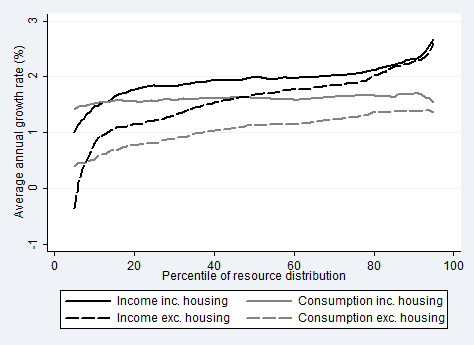
\includegraphics[width=.8\linewidth]{pictures/gic_7.png}
\label{fig:gicall}
\end{figure}

[Needs a note and source. Note that we trimmed the top and bottom 5\%].

Several stylised facts can be seen. First, income has grown by more than consumption between 1979 and 2009, other than at the bottom of the distribution (the lines cross at the Xth centile if resources include imputed income or consumption from housing, and the Yth centile if not) [Mike asks ABI: can you look these up?]. Second, over the period as a whole, measures of resources that include the imputed consumption or income from housing grew faster than those that did not. Importantly, this does not simply reflect that rental prices have increased at a faster rate than average inflation over this period: as Section \ref{measure} explains, we deflate the IHC measures of income and consumption by a variant of the RPI that weights the change in the price of rent by the budget share of actual plus \emph{imputed} rent. Instead, the fact that resources IHC have grown faster than resources XHC reflects that there has been a rise in the net housing assets owned by UK households. Third, all measures exhibit a pattern of growth that is inequality-increasing within the percentiles plotted in the figure (because growth rates rise across the distribution), but the increase in inequality is greater for income than consumption. Fourth, the growth in household resources that do not include the imputed consumption or income from housing are more inequality-increasing than those of resources that do include such (as shown by the steeper positive gradient of the GICs for the former), meaning that the imputed income or consumption from housing has an inequality-reducing effect. Indeed, the inequality-reducing effect of adding the imputed resources from housing is especially stark in the two GICs for consumption, as growth in full consumption is close to flat across the distribution.


Figure \ref{fig:gicsub} breaks the period down into six 5-year periods. Abstracting from whether growth was positive or negative, we can characterise the changes in the distribution of household resources within each of the six periods as follows:\footnote{We do not attempt to provide explanations for these changes, but see (for example) Brewer and Wren-Lewis (2015) for an assessment of why inequality in income changed over this period.} 1979-1985 saw growth that was inequality-increasing, except at the bottom (where resources at the bottom of the distribution grew by more than slightly higher up, with the four measures giving different impressions of where in the bottom half was the turning point). 1986-1990 saw growth that was strongly inequality-increasing. 1991-1995 saw growth that was slightly inequality-reducing. 1996-2000 saw growth rates that were approximately equal across the distribution, except at the bottom, where they were lower. 2001-2005 saw growth that was slightly inequality-increasing, especially at the top. 2006-2009 saw growth that was strongly inequality-reducing, except at the bottom. In general, consumption grew faster than income across most of the distribution at the start of the period (between 1979-1985 and 1986-1990), but income grew faster than consumption at the end of the period (between 2001-2005 and 2006-2009).

\begin{figure}
\caption{Growth Incidence Curves for Income and Consumption, by Sub-Period}
\centering
\begin{tabular}{cc}
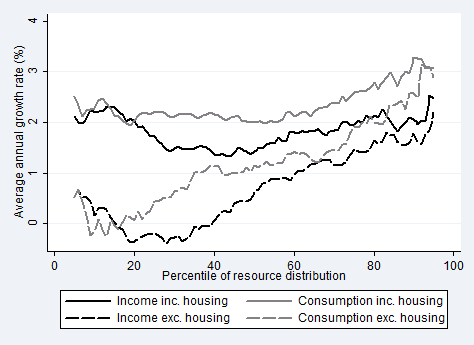
\includegraphics[width=.5\linewidth]{pictures/gic_1.png} & 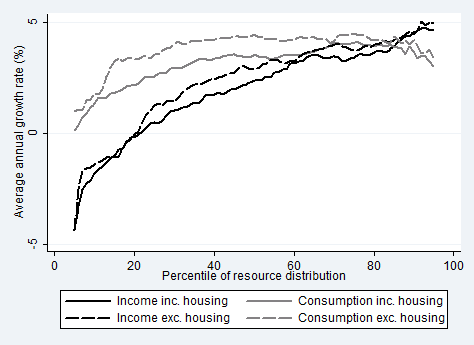
\includegraphics[width=.5\linewidth]{pictures/gic_2.png} \\
(a) 1981-1985 & (b) 1986-1990 \\
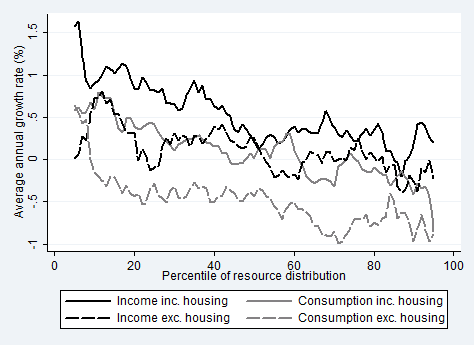
\includegraphics[width=.5\linewidth]{pictures/gic_3.png} & 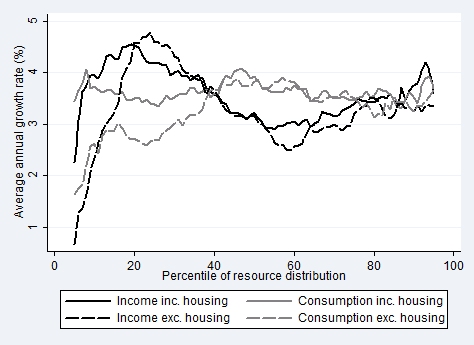
\includegraphics[width=.5\linewidth]{pictures/gic_4.png} \\
(c) 1991-1995 & (d)1996-2000 \\
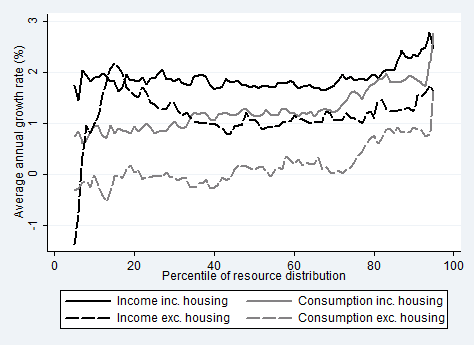
\includegraphics[width=.5\linewidth]{pictures/gic_5.png} & 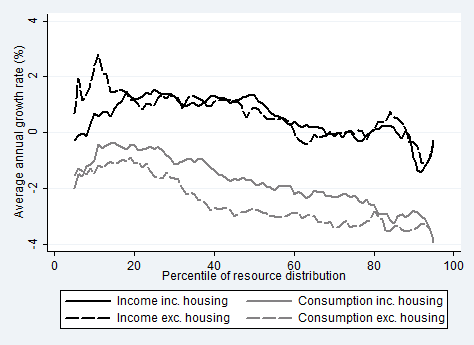
\includegraphics[width=.5\linewidth]{pictures/gic_6.png} \\
(e) 2001-2005 & (f) 2006-2009
\end{tabular}
\label{fig:gicsub}
\end{figure}

[Needs a note and source. Note that we trimmed the top and bottom 5\%].

Two sub-periods are notable for stark differences between the patterns of growth of the different resource measures: the most recent sub-period, 2006-2009, and the sub-period covering the boom of the late 1980s.  In the late 1980s, inequality in household income grew by far more than household consumption (and this is true IHC and XHC). In the late 2000s, income grew by more (or fell by less) than consumption across the whole distribution, but especially at the top, meaning that inequality in consumption looks likely to have fallen by more than inequality in income (although patterns of growth amongst the bottom 20\% were inequality-increasing). In this sub-period, moving from measuring resources that do not include the imputed consumption or income from housing to measures that do boosts growth rates across the consumption distribution, but makes little difference to inequality in household income. [NEED TO TALK HERE ABOUT FALLING COVERAGE AT THE TOP. DO WE?]


%, and that the average number of rooms per person rose from 1.93 in 1979 to 2.37 in 2000, a 23\% rise (see Figure  \ref{fig:room_time}). [Mike says: not sure about including this. Wouldn't we need to show this only for those who own property? Why not just show mean income from housing?]

%\subsection{Trends in summary measures of inequality and poverty}

%In this sub-section, we explore that the different patterns of growth in household resources, as assessed by our four measures, mean for the evolution of summary measures of inequality and poverty.

Figure \ref{fig:inequal_trends} shows trends between 1979 and 2009 in the 90-10 and 50-10 ratios, for each of the four measure of resources.\footnote{Appendix \ref{subsec:relative_poverty} analyses trends in relative poverty, defined as living in a household with less than 60\% of median income: in general, trends in this relative poverty rate are very similar to trends in the 50-10 ratio, for all measures of resources.} In general, there was little change in inequality from 1979 to the mid 1980s. As has been well-documented, there was then a sharp rise in inequality, peaking in 1989 or 1990. As we explain in detail shortly, the trends since 1990s depend on the measure used.

\begin{figure}[bp!]
\caption{Income \& Consumption Inequality, 1979-2009}
\centering
\begin{tabular}{cc}
\multicolumn{2}{c}{90-10 Ratio} \\
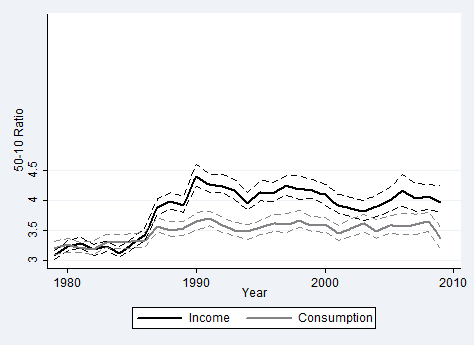
\includegraphics[width=.5\linewidth]{pictures/ihc_1.png} & 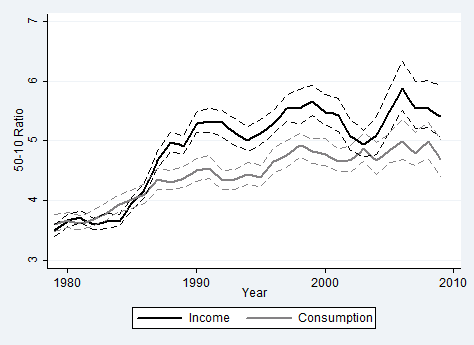
\includegraphics[width=.5\linewidth]{pictures/xhc_1.png} \\
(a) IHC & (b) XHC \\
\multicolumn{2}{c}{50-10 Ratio} \\
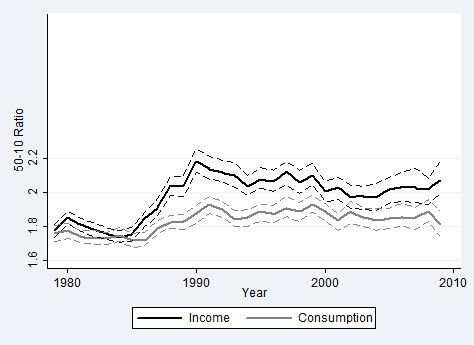
\includegraphics[width=.5\linewidth]{pictures/ihc_2.png} & 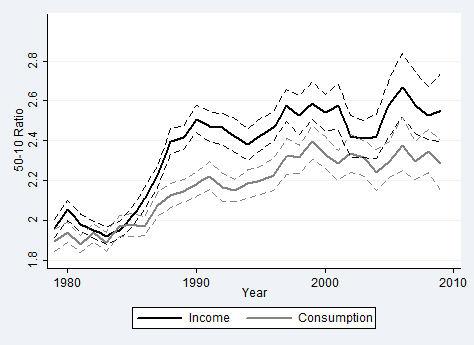
\includegraphics[width=.5\linewidth]{pictures/xhc_2.png} \\
(c) IHC & (d) XHC \\
\end{tabular}
\label{fig:inequal_trends}
\end{figure}

[NEEDS NOTE AND SOURCE. \footnote{Confidence intervals are obtained as $\hat{\mu} + 1.96se(\hat{\mu})$, where $se(\hat{\mu})$ is calculated from the bootstrap distribution of the relevant statistic obtained from 1,000 random draws with replacement independently for each year.}]

As would expected given the difference in the GICs shown in Figure \ref{fig:gicall}, income and consumption give different impressions of how inequality has changed between 1979 and 2009.  First, since the mid 1980s, inequality have been higher when assessed using income, rather than consumption. In particular, and as shown by sub-panel (b) of Figure \ref{fig:gicsub}, the rise in inequality in the late 1980s is much more dramatic when assessed with income than with consumption. If we do not include the imputed resources from housing, then inequality has risen faster since 1990 when assessed using consumption than when assessed using income; if we do include the imputed resources from housing, then there has been little difference in the post-1990s trends in inequality in income and consumption. It is also clear that the measures of resources that do include the imputed resources from housing are more equally distributed, particularly at the bottom, than those that do not, underscoring the fact that the imputed resources derived from housing are more equally distributed than other resources. Furthermore, this inequality-reducing effect of adding the imputed resources from housing is growing over time, so that the post-1990s trends in inequality in resources that do include imputed resources from housing are broadly flat (consumption) or falling (income), but the post-1990s trends in inequality in resources that do not include imputed resources from housing are rising (both income and consumption).


%\subsection{Relative poverty using income and consumption}\label{subsec:relative_poverty}

Figure \ref{fig:pov_trends} shows trends in a measure of relative poverty (defined as having a level of resources below 60\% of the contemporaneous median resource measure), for each of the four measure of resources. In general, there was little change in relative poverty from 1979 to the mid 1980s, followed by a sharp rise, peaking in 1989 or 1990. 

\begin{figure}
\caption{Rates of Relative Poverty, 1979-2009}
\centering
\begin{tabular}{cc}
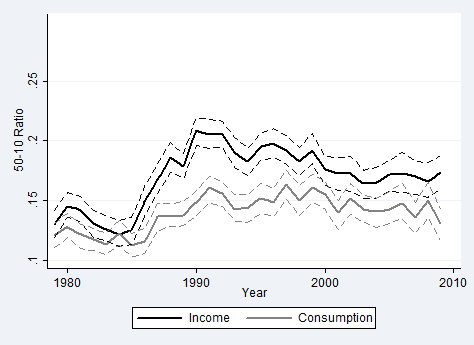
\includegraphics[width=.5\linewidth]{pictures/ihc_3.png} & 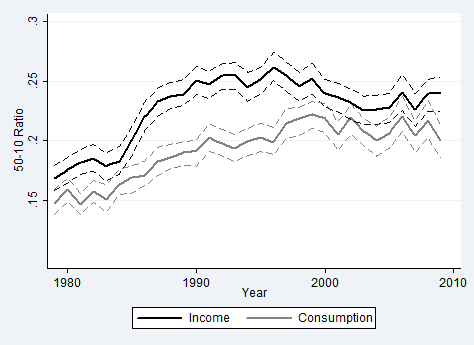
\includegraphics[width=.5\linewidth]{pictures/xhc_3.png} \\
(a) IHC & (b) XHC \\
\end{tabular}
\label{fig:pov_trends}
\end{figure}

[NEEDS NOTE AND SOURCE. \footnote{Confidence intervals are obtained as $\hat{\mu} + 1.96se(\hat{\mu})$, where $se(\hat{\mu})$ is calculated from the bootstrap distribution of the relevant statistic obtained from 1,000 random draws with replacement independently for each year.}]



\subsection{Rank correlations between income and consumption}\label{subsec:ranks}

%[THIS DOESN'T QUITE FIT HERE (IT's NOT ABOUT POVERTY). I AM WONDERING WHETHER TO PUT IN INTO AN ANNEX?]

Table \ref{table:kendall} shows the similarity of the orderings of households given by our four measures of resources by showing the Kendall rank correlation coefficient, $\tau$, for the selection of years shown in Table \ref{table:prctile}.\footnote{For any two pairs of ranks $(x_{i},y_{i})$ and $(x_{j},y_{j})$ of a variable pair $(x, y)$, define them as concordant if: $(x_{i}-x_{j})(y_{i} - y_{j}) > 0$ and discordant otherwise. Kendall's score is then defined as $\tau = \frac{C-D}{\frac{1}{2}n(n-1)}$, where $C$ is the number of concordant pairs and $D$ is the number of discordant pairs.}

Although there is positive agreement between the rankings (i.e. $\tau>0$ for all pairwise comparisons), all measures give different rankings (i.e. $\tau<1$ for all pairwise comparisons). For the measures that do not include imputed resources from housing, $\tau$ has fallen from 0.49 in 1979 to 0.43 in 2009. Unsurprisingly, $\tau$ for the measures that do include imputed resources from housing is slightly higher (reflecting that both measures contain a identical component equal to the imputed resources from housing); more interestingly, it also shows no clear pattern over time, fluctuating between 0.48 and 0.51.

The values of $\tau$ for pairs of measures that do and do not include the imputed income from housing are, unsurprisingly, much higher, but have also fallen over time, from 0.90 to 0.82 for the two measures of income, and from 0.90 to 0.75 for the two measures of consumption. This reflects a rise over time in the implicit resources from housing that is not perfectly aligned with one's position in the without-housing-resources distribution (and this in turn echoes the finding of Figure \ref{fig:gicall} that the inequality-reducing impact of including resources from housing in a measure of consumption is increasing over time.

\begin{table}[tp!]
\caption{Rank Correlation Between Resource Measures: Kendall's Tau}
\centering
\begin{tabular}{lcccc}
\hline\hline 	
 &  Income IHC & Cons. IHC & Income XHC & Cons. XHC \\
\hline
\multicolumn{5}{l}{\textbf{1979}}  \\
Income IHC &1.0000$^{***}$ & & & \\
 & (0.000)  & & & \\
Cons. IHC & 0.4877$^{***}$&1.0000$^{***}$ & & \\
 & (0.000) &(0.000) & & \\
Income XHC & 0.9006$^{***}$&0.4716$^{***}$ &1.0000$^{***}$ & \\
  & (0.000) &(0.000) & (0.000) & \\
Cons. XHC &0.4733$^{***}$ &0.8980$^{***}$ &0.4890$^{***}$ &1.0000$^{***}$ \\
 & (0.000) &(0.000) & (0.000) & (0.000) \\
\hline
\multicolumn{5}{l}{\textbf{2009}}  \\
Income IHC &1.0000$^{***}$ & & & \\
 & (0.000)  & & & \\
Cons. IHC & 0.4755$^{***}$&1.0000$^{***}$ & & \\
 & (0.000) &(0.000) & & \\
Income XHC & 0.8202$^{***}$&0.3956$^{***}$ &1.0000$^{***}$ & \\
  & (0.000) &(0.000) & (0.000) & \\
Cons. XHC &0.4066$^{***}$ &0.7574$^{***}$ &0.4281$^{***}$ &1.0000$^{***}$ \\
 & (0.000) &(0.000) & (0.000) & (0.000) \\
\hline\hline
\multicolumn{5}{l}{Notes: p-values in brackets. }
\end{tabular}
\label{table:kendall}
\end{table}


\subsection{NEEDS A TITLE}

[Mike says: these are all out of date: we have changed the specification since these were done].

This appendix presents variants to Tables \ref{table:multinom_incon} and \ref{table:ahc_bhc} for the earlier two decades.

%\footnotesize

\begin{table}
\caption{Income versus Consumption: 1990-1989}
\centering
\begin{tabular}{l|ccc|ccc}
\hline\hline 
	& \multicolumn{3}{c}{\textbf{BHC Bottom Decile}} &  \multicolumn{3}{c}{\textbf{AHC. Bottom Decile}} \\
	&	$r_{IC}$	&	$r_{I}$	&	$r_{C}$	&	$r_{IC}$	&	$r_{I}$	&	$r_{C}$	\\
  & se & se & se  & se & se & se \\
\hline
Left school $\leq$ 16	&	       2.446***	&	       1.371***	&	       2.828***	&	       1.369***	&	1.064	&	       1.864***	\\				
                    	&	       0.429   	&	0.072	&	0.38	&	       0.112   	&	0.044	&	0.074	\\				
Left school $>$ 19	&	       0.799   	&	       0.869*  	&	       0.654***	&	       0.822   	&	0.947	&	       0.801*  	\\				
                    	&	       0.161   	&	0.056	&	0.066	&	       0.133   	&	0.051	&	0.077	\\				
Age $<$ 30	&	       1.076   	&	       1.195** 	&	0.946	&	       1.190** 	&	       1.226***	&	       0.759*  	\\				
                    	&	       0.087   	&	0.072	&	0.09	&	       0.074   	&	0.054	&	0.088	\\				
Age 30-40	&	       1.133   	&	       1.162** 	&	       1.236*  	&	       1.021   	&	1.07	&	1.081	\\				
                    	&	       0.081   	&	0.057	&	0.126	&	       0.087   	&	0.057	&	0.138	\\				
Age 50-60	&	       0.826   	&	       0.846** 	&	1.125	&	       0.855   	&	0.922	&	1.085	\\				
                    	&	       0.103   	&	0.048	&	0.089	&	       0.121   	&	0.065	&	0.097	\\				
Age 60-70	&	       0.376***	&	       0.424***	&	       1.376** 	&	       0.149***	&	       0.368***	&	1.146	\\				
                    	&	       0.049   	&	0.03	&	0.145	&	       0.019   	&	0.032	&	0.135	\\				
Age $\geq$ 70	&	       0.424***	&	       0.233***	&	       2.399***	&	       0.233***	&	       0.226***	&	       2.183***	\\				
                    	&	       0.053   	&	0.025	&	0.286	&	       0.036   	&	0.024	&	0.294	\\				
Unemployed	&	       7.997***	&	       4.224***	&	       2.517***	&	      10.829***	&	       4.365***	&	       3.137***	\\				
	&	       0.918   	&	0.254	&	0.094	&	       1.296   	&	0.291	&	0.14	\\				
Constant            	&	       0.014***	&	       0.028***	&	       0.026***	&	       0.014***	&	       0.040***	&	0.179	\\				
                    	&	       0.003   	&	0.002	&	0.004	&	       0.002   	&	0.004	&	       2.801***	\\
\hline\hline
\multicolumn{7}{l}{Significantly different from zero at the 5\% ($\star\star$) and 1\% level ($\star\star\star$).} \\
\multicolumn{7}{l}{Omitted variables: Left school between 17-18 years old, household head aged between} \\
\multicolumn{7}{l}{40 and 50 years, employed. Controls for household composition.}
\end{tabular}
\end{table}

\begin{table}
\caption{Income versus Consumption: 1980-1989}
\centering
\begin{tabular}{l|ccc|ccc}
\hline\hline 
	& \multicolumn{3}{c}{\textbf{BHC Bottom Decile}} &  \multicolumn{3}{c}{\textbf{AHC. Bottom Decile}} \\
	&	$r_{IC}$	&	$r_{I}$	&	$r_{C}$	&	$r_{IC}$	&	$r_{I}$	&	$r_{C}$	\\
  & se & se & se  & se & se & se \\
\hline
Left school $\leq$ 16	&	       2.171***	&	       1.233** 	&	       2.025***	&	       1.603***	&	       1.137*  	&	       2.123***	\\				
                    	&	       0.270   	&	0.079	&	0.192	&	       0.199   	&	0.06	&	0.144	\\				
Left school $>$ 19	&	       0.615*  	&	       0.815*  	&	0.681	&	       0.597** 	&	0.919	&	0.835	\\				
                    	&	       0.140   	&	0.071	&	0.149	&	       0.116   	&	0.046	&	0.107	\\				
Age $<$ 30	&	       0.918   	&	       1.294***	&	0.965	&	       0.980   	&	       1.346***	&	1.163	\\				
                    	&	       0.081   	&	0.078	&	0.081	&	       0.131   	&	0.078	&	0.124	\\				
Age 30-40	&	       1.070   	&	1.026	&	1.188	&	       0.873   	&	0.98	&	1.143	\\				
                    	&	       0.095   	&	0.075	&	0.108	&	       0.101   	&	0.065	&	0.097	\\				
Age 50-60	&	       0.757*  	&	0.892	&	0.873	&	       0.809   	&	       0.830** 	&	0.825	\\				
                    	&	       0.087   	&	0.073	&	0.169	&	       0.089   	&	0.053	&	0.146	\\				
Age 60-70	&	       0.404***	&	       0.536***	&	       1.488** 	&	       0.236***	&	       0.372***	&	       1.459** 	\\				
                    	&	       0.034   	&	0.073	&	0.188	&	       0.039   	&	0.044	&	0.174	\\				
Age $\geq$ 70	&	       0.639***	&	       0.370***	&	       3.077***	&	       0.369***	&	       0.254***	&	       3.107***	\\				
                    	&	       0.064   	&	0.041	&	0.297	&	       0.056   	&	0.028	&	0.297	\\				
Unemployed	&	      13.615***	&	       6.035***	&	       2.510***	&	      18.302***	&	       7.111***	&	       3.140***	\\				
                    	&	       0.901   	&	0.858	&	0.121	&	       1.212   	&	0.828	&	0.104	\\				
Constant            	&	       0.004***	&	       0.015***	&	       0.013***	&	       0.004***	&	       0.018***	&	       0.011***	\\				
                    	&	       0.001   	&	0.002	&	0.002	&	       0.001   	&	0.003	&	0.002	\\
\hline\hline
\multicolumn{7}{l}{Significantly different from zero at the 5\% ($\star\star$) and 1\% level ($\star\star\star$).} \\
\multicolumn{7}{l}{Omitted variables: Left school between 17-18 years old, household head aged between} \\
\multicolumn{7}{l}{40 and 50 years, employed. Controls for household composition.}
\end{tabular}
\end{table}

\begin{table}
\caption{AHC versus BHC: 1990-1999}
\centering
\begin{tabular}{l|ccc|ccc}
\hline\hline 
	& \multicolumn{3}{c}{\textbf{Income Bottom Decile}} &  \multicolumn{3}{c}{\textbf{Cons. Bottom Decile}} \\
	&	$r_{AB}$	&	$r_{A}$	&	$r_{B}$	&	$r_{AB}$	&	$r_{A}$	&	$r_{B}$	\\
  & se & se & se  & se & se & se \\
\hline
Left school $\leq$ 16	&	       1.226***	&	       2.486***	&	       0.700***	&	       2.390***	&	       2.891***	&	1.054	\\
                    	&	       0.055   	&	0.216	&	0.072	&	       0.265   	&	0.363	&	0.083	\\
Left school $>$ 19	&	       0.860** 	&	       0.526***	&	1.041	&	       0.709*  	&	       0.497***	&	0.877	\\
                    	&	       0.045   	&	0.066	&	0.134	&	       0.102   	&	0.079	&	0.153	\\
Age $<$ 30	&	       1.486***	&	1.096	&	       1.435***	&	       1.181*  	&	1.207	&	1.073	\\
                    	&	       0.089   	&	0.106	&	0.133	&	       0.098   	&	0.122	&	0.099	\\
Age 30-40	&	       1.294***	&	       1.526***	&	1.023	&	       1.406***	&	       1.651***	&	1.104	\\
                    	&	       0.063   	&	0.128	&	0.091	&	       0.126   	&	0.108	&	0.172	\\
Age 50-60	&	       0.725***	&	       0.368***	&	0.979	&	       0.766*  	&	       0.621***	&	       1.320** 	\\
                    	&	       0.035   	&	0.054	&	0.115	&	       0.079   	&	0.039	&	0.118	\\
Age 60-70	&	       0.274***	&	       0.270***	&	       0.354***	&	       0.583***	&	       0.493***	&	1.103	\\
                    	&	       0.016   	&	0.043	&	0.047	&	       0.073   	&	0.036	&	0.155	\\
Age $\geq$ 70	&	       0.159***	&	       0.259***	&	       0.364***	&	       1.155   	&	       0.658***	&	       2.205***	\\
                    	&	       0.016   	&	0.041	&	0.046	&	       0.161   	&	0.043	&	0.295	\\
Unemployed	&	       5.249***	&	       6.063***	&	       7.492***	&	       4.816***	&	       3.289***	&	       4.494***	\\
	&	       0.336   	&	0.51	&	0.406	&	       0.289   	&	0.255	&	0.366	\\
Constant            	&	       0.075***	&	       0.024***	&	       0.051***	&	       0.053***	&	       0.029***	&	       0.044***	\\
                    	&	       0.006   	&	0.003	&	0.008	&	       0.008   	&	0.003	&	0.007	\\
\hline\hline
\multicolumn{7}{l}{Significantly different from zero at the 5\% ($\star\star$) and 1\% level ($\star\star\star$).} \\
\multicolumn{7}{l}{Omitted variables: Left school between 17-18 years old, household head aged between} \\
\multicolumn{7}{l}{40 and 50 years, employed. Controls for household composition.} 
\end{tabular}
\end{table}

\begin{table}
\caption{AHC versus BHC: 1980-1989}
\centering
\begin{tabular}{l|ccc|ccc}
\hline\hline 
	& \multicolumn{3}{c}{\textbf{Income Bottom Decile}} &  \multicolumn{3}{c}{\textbf{Cons. Bottom Decile}} \\
	&	$r_{AB}$	&	$r_{A}$	&	$r_{B}$	&	$r_{AB}$	&	$r_{A}$	&	$r_{B}$	\\
  & se & se & se  & se & se & se \\
\hline
Left school $\leq$ 16	&	       1.198** 	&	       1.985***	&	0.874	&	       2.237***	&	       2.019***	&	       1.230*  	\\
                    	&	       0.077   	&	0.165	&	0.096	&	       0.184   	&	0.257	&	0.112	\\
Left school $>$ 19	&	       0.822** 	&	       0.582*  	&	1.1	&	       0.706   	&	0.677	&	1.078	\\
                    	&	       0.055   	&	0.13	&	0.158	&	       0.163   	&	0.185	&	0.21	\\
Age $<$ 30	&	       1.624***	&	       1.206*  	&	       1.800***	&	       1.289** 	&	1.047	&	       1.376*  	\\
                    	&	       0.102   	&	0.107	&	0.188	&	       0.124   	&	0.096	&	0.216	\\
Age 30-40	&	       1.354***	&	       1.618***	&	1.204	&	       1.427***	&	       1.603***	&	1.022	\\
                    	&	       0.089   	&	0.139	&	0.127	&	       0.123   	&	0.092	&	0.139	\\
Age 50-60	&	       0.687***	&	       0.495***	&	1.012	&	       0.754*  	&	       0.499***	&	1.159	\\
                    	&	       0.032   	&	0.043	&	0.073	&	       0.102   	&	0.052	&	0.113	\\
Age 60-70	&	       0.346***	&	       0.455***	&	       0.584** 	&	       0.928   	&	       0.517***	&	       1.505***	\\
                    	&	       0.040   	&	0.047	&	0.109	&	       0.088   	&	0.042	&	0.134	\\
Age $\geq$ 70	&	       0.265***	&	       0.601***	&	       0.650*  	&	       2.193***	&	       0.793***	&	       2.967***	\\
                    	&	       0.037   	&	0.07	&	0.111	&	       0.199   	&	0.041	&	0.275	\\
Unemployed	&	       8.440***	&	       7.189***	&	      12.197***	&	       4.969***	&	       4.038***	&	       5.608***	\\
	&	       0.903   	&	0.451	&	0.738	&	       0.210   	&	0.277	&	0.396	\\
Constant            	&	       0.051***	&	       0.014***	&	       0.024***	&	       0.028***	&	       0.020***	&	       0.018***	\\
                    	&	       0.006   	&	0.002	&	0.005	&	       0.003   	&	0.002	&	0.003	\\
\hline\hline
\multicolumn{7}{l}{Significantly different from zero at the 5\% ($\star\star$) and 1\% level ($\star\star\star$).} \\
\multicolumn{7}{l}{Omitted variables: Left school between 17-18 years old, household head aged between} \\
\multicolumn{7}{l}{40 and 50 years, employed. Controls for household composition.} \end{tabular}
\end{table}

